% book of real analysis exercises
% nicola frosi
% starting date 18-05-2024

\documentclass[a4paper, twoside, openany]{book}

\usepackage[utf8]{inputenc}
\usepackage[T1]{fontenc}
\usepackage[english]{babel}

\usepackage[margin=2.5 cm]{geometry}

\usepackage{float}
\usepackage{rotating}


\usepackage{amsmath}
\usepackage{amsfonts}
\usepackage{amssymb}
\usepackage{amsthm}

\usepackage{tikz}
\usetikzlibrary{arrows.meta, calc, quotes}
\usepackage{pgfplots}

\newcommand{\norm}[1]{\left\lVert#1\right\rVert}
\newcommand{\esssup}{\operatornamewithlimits{ess\,sup}}
\newcommand\bigfrown[2][\textstyle]{\ensuremath{%
  \array[b]{c}\text{\scalebox{2}{$#1\frown$}}\\[-1.3ex]#1#2\endarray}}

\title{\textbf{\huge{\textit{A collection of Real Analysis exercises}}}}

\begin{document}
\maketitle
\chapter{Metric Spaces}
\section*{Exercise $1$}
Let the  distances in $\mathbb{R}^2$:
\begin{enumerate}
\item $d_1(X, Y) = \sum_{i=1}^2 |y_i - x_i| = |y_1 - x_1| + |y_2 - x_2|$;
\item $d_2(X, Y) = \sqrt{\sum_{i=1}^2 |y_i -x_i|^2} = \sqrt{|y_1 - x_1|^2 + |y_2 - x_2|^2}$;
\item $d_{\infty}(X, Y) = \max_{i=1,2} |y_i - x_i| = \max \{ |y_1 - x_1|, |y_2 - x_2| \}$. 
\end{enumerate}
Construct the open balls related to these distances.
\section*{Solution}
\textbf{Point $1$} 
$$d_1(X, Y) < r$$
$$\textrm{iff}$$
$$\sum_{i=1}^2 |y_i - x_i| < r$$
$$\textrm{iff}$$
$$|y_1 - x_1| + |y_2 - x_2| < r$$
\begin{figure}[!ht]
\begin{center}
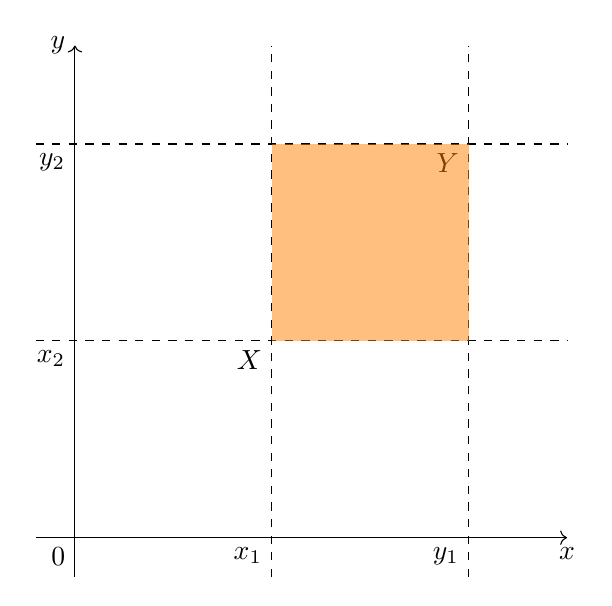
\begin{tikzpicture}[scale=2.5]
\draw[->] (-0.2,0)--(2.5,0) node[below]{$x$};   
\draw[->] (0,-0.2)--(0,2.5)  node[left]{$y$};
\draw[dashed] (1,-0.2)--(1,2.5);
\draw[dashed] (2,-0.2)--(2,2.5);
\draw[dashed] (-0.2,1)--(2.5,1);
\draw[dashed] (-0.2,2)--(2.5,2);
\path
(0,0) node[below left]{$0$};
\path
(1,1) node[below left]{$X$};
\path
(2,2) node[below left]{$Y$};
\path
(0,1) node[below left]{$x_2$};
\path
(1,0) node[below left]{$x_1$};
\path
(2,0) node[below left]{$y_1$};
\path
(0,2) node[below left]{$y_2$};
\path [fill=orange, opacity=0.5] (1.,1.) rectangle (2.,2.);
\end{tikzpicture}
\end{center}
\end{figure}
\textbf{Point $2$}
$$d_2(X;Y) < r$$
$$\textrm{iff}$$
$$\sqrt{|y_1 - x_1|^2 + |y_2 - x_2|^2} < r$$
$$\textrm{iff}$$
$$|y_1 - x_1|^2 + |y_2 - x_2|^2 < r^2$$
\begin{figure}[!ht]
\begin{center}
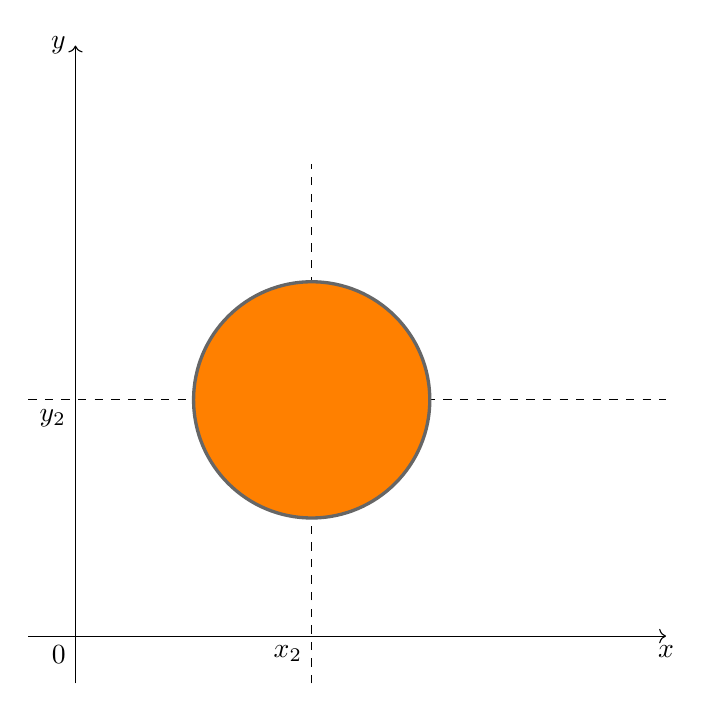
\begin{tikzpicture}[scale=3.]
\draw[->] (-0.2,0)--(2.5,0) node[below]{$x$};   
\draw[->] (0,-0.2)--(0,2.5)  node[left]{$y$};
\draw[dashed] (-0.2,1)--(2.5,1);
\draw[dashed] (1,-0.2)--(1,2);
\path
(0,0) node[below left]{$0$};
\path
(1,0) node[below left]{$x_2$};
\path
(0,1) node[below left]{$y_2$};
\filldraw[color=black!60, fill=orange, very thick](1,1) circle (0.5);
\end{tikzpicture}
\end{center}
\end{figure}
\textbf{Point $3$}
$$d_{\infty}(X, Y) < r$$
$$\textrm{iff}$$
$$\max \{ |y_1 - x_1|, |y_2 - x_2| \}$$
\begin{figure}[!ht]
\begin{center}
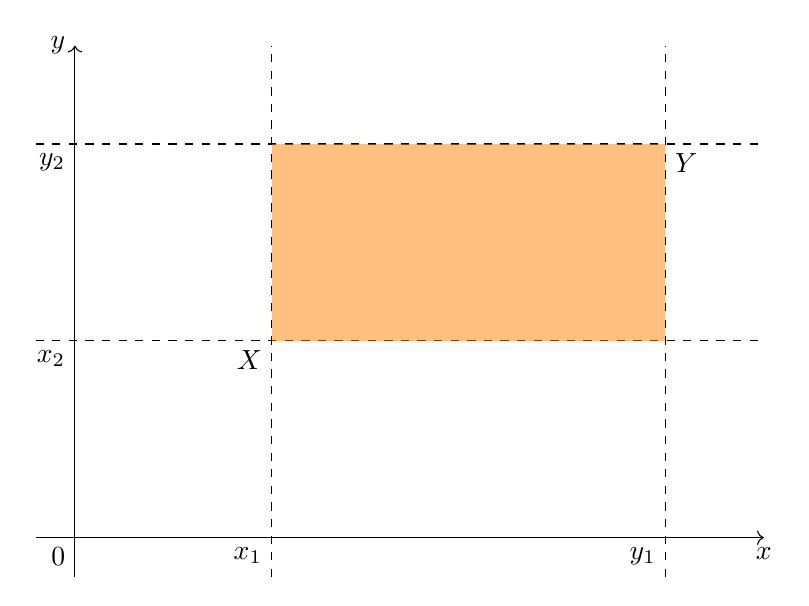
\begin{tikzpicture}[scale=2.5]
\draw[->] (-0.2,0)--(3.5,0) node[below]{$x$};   
\draw[->] (0,-0.2)--(0,2.5)  node[left]{$y$};
\draw[dashed] (1,-0.2)--(1,2.5);
\draw[dashed] (3,-0.2)--(3,2.5);
\draw[dashed] (-0.2,1)--(3.5,1);
\draw[dashed] (-0.2,2)--(3.5,2);
\path
(0,0) node[below left]{$0$};
\path
(1,1) node[below left]{$X$};
\path
(3,2) node[below right]{$Y$};
\path
(0,1) node[below left]{$x_2$};
\path
(1,0) node[below left]{$x_1$};
\path
(3,0) node[below left]{$y_1$};
\path
(0,2) node[below left]{$y_2$};
\path [fill=orange, opacity=0.5] (1.,1.) rectangle (3.,2.);
\end{tikzpicture}
\end{center}
\end{figure}
\clearpage
\section*{Exercise $2$}
Let $(X, d)$ a metric space, $A \subset X$ not empty. Show if the following statements are true or false:
\begin{enumerate}
\item $A \qquad \textrm{open} \qquad \implies \mathring{A} \cap \partial A = \emptyset$;
\item if $\mathring{A} \cap \partial A = \emptyset \implies A \qquad \textrm{closed}$;
\end{enumerate}
\section*{Solution}
\textbf{Point $1$} \par 
The first statement is always true. It is also true if $A$ is closed or if $A$ is neither open or closed.
$$\partial A = \{ x \in X \textrm{s.t.} x \notin \mathring{A} \qquad \textrm{and} \qquad x \notin \mathring{\bigfrown{X \setminus A}} \}$$
$$\implies \mathring{A} \cap \partial A = \emptyset \qquad \textrm{is} \qquad \textrm{true}.$$
\textbf{Point $2$} \par  
The second statement is false. Counterexample:
$$A = ]0, 1[$$
is an open set with
$$\partial A = \{ 0, 1 \}$$
and we have that $\mathring{A} \cap \partial A = \emptyset \implies A \qquad \textrm{is} \qquad \textrm{closed}$ is false because $A$ is open.
\clearpage
\section*{Exercise $3$}
Let $(X, d)$ a metric space $A \subset X$ closed and $A \neq \emptyset$. Furthermore let
$$f: X \rightarrow \mathbb{R}$$
with
$$f(x) = \inf_{a \in A \setminus \{ x \}} d(x, a).$$
Tell wether the following statements are true or false.
\begin{enumerate}
\item $x \in A \implies f(x) = 0$;
\item $f(x) = 0 \implies x \in A$;
\end{enumerate}
\section*{Solution}
\textbf{Point $1$} \par  
This statement is not true $\forall x$. Counterexample:
$$A = [0, 1] \cup \{ 2 \}$$
we have that $2 \in A$, but $f(2) \neq 0$ because $f(2) = \inf d(2, a)$ with $a \in [0, 1]$. If $a \in [0,1]$ the distance of $2$ from $a$ is greater(or equal) than the distance of $2$ from $1$.
$$\textrm{If} \qquad a \in [0, 1]$$
$$\textrm{then} d(2, a) \geq d(2, 1) = 1$$
so that
$$\textrm{if} d(2, a) \geq 1 \implies \forall a \in [0, 1] \qquad d(2, a) \geq 1.$$
Then
$$\inf d(2, a) \geq 1 \qquad a \in [0, 1]$$
and it can't be equal to zero. \par 
\textbf{Point $2$} \par   
Remeber that $x$ is an accumulation point for $A$ iff $\inf_{a \in A \setminus \{ x \}} d(x, a) = 0$.
$$f(x) = 0 \implies x \qquad \textrm{is an accumulation point for A}$$
$$\textrm{then} \qquad x \in \overline{A} = A \qquad \textrm{since A is closed}$$
then the second statement is true.
\clearpage
\section*{Exercise $4$}
Let $X = C^0([0, 1])$, $d_{\infty}(f, g) = \sup_{t \in [0,1]} |f(t) - g(t)|$ and $d_2(f, g) = \sqrt{\int_0^1 |f(t) - g(t)|^2 dt}$. Show that $d_2$ and $d_{\infty}$ are not equivalent.
\section*{Solution}
If we choose $f_n(t) = t^n \qquad \forall n \in \mathbb{N}$, we have that:
$$d_{\infty}(f_n, 0) = \sup_{t \in [0, 1]} |f_n(t)| = \sup_{t \in [0, 1]} |t^n| = 1.$$
It is a maximum.
$$(d_2(f_n, 0))^2 = \int_0^1 |f_n(t)|^2 dt = \int_0^1 (t)^{2 n} dt = [ \frac{t^{2n + 1}}{2n + 1}]_0^1 = \frac{1}{2n + 1}$$
then
$$d_2(f_n, 0) = \frac{1}{2n + 1}$$
for $n \rightarrow \infty$, $d_2 \rightarrow 0$. So that
$$\forall c \in \mathbb{R} \exists n \in \mathbb{N} \qquad \textrm{s.t.} \qquad d_{\infty}(f_n, 0) > c d_2(f_n, 0)$$
then $d_2$ and $d_{\infty}$ are not equivalent.
\clearpage
\section*{Exercise $5$}
Let $X = C^0([0, 1])$. Show that the open ball $B_{d_2}(0,1)$ is unbounded with respect to $d_{\infty}$.
\section*{Solution}
Consider the following sequence of functions:
$$f_n(t) = \begin{cases}
			-n^{\frac{5}{4}}(t - \frac{1}{n}) \qquad \textrm{for} \qquad t \in [0, \frac{1}{n}] \\
			0 \qquad \textrm{for} \qquad t \in ]\frac{1}{n}, 1]
		   \end{cases}$$
\begin{figure}[!ht]
\begin{center}
\begin{tikzpicture}[scale=6.]
\draw[->] (-0.5,0)--(1.5,0) node[below]{$t$};   
\draw[->] (0,-0.5)--(0,1.5)  node[left]{$f_n$};
\draw[dashed] (1,-0.5)--(1,1.5);
\path
(0,0) node[below left]{$0$};
\path
(1,0) node[below left]{$1$};
\foreach \i in {0.,0.1, 0.2,...,1.0} \draw (\i,-0.02)--(\i,0.02);
\draw[blue, domain=0.:1., samples=100, variable=\x] plot ({\x}, {-(\x - 1)});
\draw[green, domain=0.:1./2, samples=100, variable=\x] plot ({\x}, {-2^(5./4)*(\x - 1./2)});
\draw[green, domain=1./2.:1., samples=100, variable=\x] plot ({\x}, {0.});
\draw[orange, domain=0.:1./3, samples=100, variable=\x] plot ({\x}, {-3^(5./4)*(\x - 1./3)});
\draw[orange, domain=1./3.:1., samples=100, variable=\x] plot ({\x}, {0.});
\draw[red, domain=0.:1./4, samples=100, variable=\x] plot ({\x}, {-4^(5./4)*(\x - 1./4)});
\draw[red, domain=1./4.:1., samples=100, variable=\x] plot ({\x}, {0.});
\end{tikzpicture}
\end{center}
\end{figure} \vspace{1 cm}
$$d_2(f, g) = \sqrt{\int_0^1 |g(t) - f(t)|^2 dt}$$
$$d_{\infty}(f_n, 0) = \sup_{t \in [0, 1]} |f_n(t)| = f_n(0) = \sqrt[4]{n} \rightarrow \infty$$
$$(d_2(f_n, 0))^2 = \int_0^{\frac{1}{n}} -n^{\frac{5}{2}}(t - \frac{1}{n}) dt = [-\frac{n^{\frac{5}{2}}}{3}(t - \frac{1}{n})^3]_0^{\frac{1}{n}} = \frac{n^{\frac{5}{2}}}{3}\frac{1}{n^3} = \frac{1}{3 \sqrt{n}}$$
then
$$d_s(f_n, 0) = \frac{1}{\sqrt{3}\sqrt{n}}.$$
With respect to $d_{\infty}$ the function is unbounded because contains a sequence the goes to infinity.
\clearpage
\section*{Exercise $6$}
Say if $[0, +\infty[$ is bounded in $(\mathbb{R}, d_0)$ and in $(\mathbb{R}, d)$, with
\begin{itemize}
\item $d_0$ the discrete metric;
\item $d$ the Euclidean metric;
\end{itemize}
\section*{Solution}
The discrete metric is characterized by the fact that the distance between two points is equal to zero or one.
$$d_0(x,y) = \begin{cases}
			1 \qquad \textrm{if} \qquad x \neq y \\
			0 \qquad \textrm{if} \qquad x = y
			\end{cases}$$
so that
$$diam([0, +\infty[) = \sup_{x,y \in [0, +\infty[} d_0(x, y) \leq 1,$$
then $[0, +\infty[$ is bounded in $(\mathbb{R}, d_0)$. \par 
If we consider the Euclidean distance
$$diam([0, +\infty[) = \sup_{x, y \in [0, +\infty[} d(x, y) = \sup_{x, y \in [0, +\infty[} |y - x| \geq n \qquad \forall n \in \mathbb{N},$$
then $diam([0, +\infty[) = + \infty$, so that $[0, +\infty[$ is unbounded with $d$.
\clearpage
\section*{Exercise $7$}
Let $(X, d)$ a metric space, $f: X \rightarrow \mathbb{R}$ a continous function and $A \subset X$ bounded. Say if the following statements are true or false.
\begin{enumerate}
\item $f(A)$ is connected;
\item $f(A)$ is compact;
\item $f(A)$ is open;
\end{enumerate}
\section*{Solution}
\textbf{Point $1$} \par   
Consider $f: \mathbb{R} \rightarrow \mathbb{R}$ given by
$$f(x) = x$$
and consider $A = [0, 1] \cup [2,3]$, there is no request on $A$, so that
$$f(A) = [0, 1] \cup [2,3]$$
is not connected.
\begin{figure}[!ht]
\begin{center}
\begin{tikzpicture}[scale=2.]
\draw[->] (-2.5,0)--(4.5,0) node[below]{$t$};   
\draw[->] (0,-2.5)--(0,4.5)  node[left]{$f_n$};
\draw[dashed] (1,-2.5)--(1,4.5);
\draw[dashed] (2,-2.5)--(2,4.5);
\draw[dashed] (3,-2.5)--(3,4.5);
\draw[dashed] (-2.5,1.)--(4.5,1.);
\draw[dashed] (-2.5,2.)--(4.5,2.);
\draw[dashed] (-2.5,3.)--(4.5,3.);
\draw[line width=5., red] (0.,0.)--(0.,1.);
\draw[line width=5., red] (0.,2.)--(0.,3.);
\path
(0,0) node[below left]{$0$};
\path
(1,0) node[below left]{$1$};
\path
(2,0) node[below left]{$2$};
\path
(3,0) node[below left]{$3$};
\path
(-0.5,2.5) node[below left]{$f(A)$};
\foreach \i in {0.,0.1, 0.2,...,3.0} \draw (\i,-0.02)--(\i,0.02);
\draw[blue, domain=-2.:4., samples=100, variable=\x] plot ({\x}, {\x});
\end{tikzpicture}
\end{center}
\end{figure} \vspace{1 cm}
\textbf{Point $2$} \par 
Consider $f: ]0, +\infty[ \rightarrow \mathbb{R}$, given by
$$f(x) = \frac{1}{x}$$
\begin{figure}[!ht]
\begin{center}
\begin{tikzpicture}[scale=2.]
\draw[->] (-2.5,0)--(4.5,0) node[below]{$t$};   
\draw[->] (0,-2.5)--(0,4.5)  node[left]{$f_n$};
\path
(0,0) node[below left]{$0$};
\path
(1,0) node[below left]{$1$};
\path
(2,0) node[below left]{$2$};
\path
(3,0) node[below left]{$3$};
\path
(-0.5,2.5) node[below left]{$f(A)$};
\foreach \i in {0.,0.1, 0.2,...,3.0} \draw (\i,-0.02)--(\i,0.02);
\draw[blue, domain=0.2:4., samples=100, variable=\x] plot ({\x}, {1. / \x});
\end{tikzpicture}
\end{center}
\end{figure} \vspace{1 cm}
If we choose $A = ]0, 1]$ we have $f(a) = [1, +\infty[$ that is not compact because it is not bounded. \par  
\textbf{Point $3$} \par  
If we consider $f: \mathbb{R} \rightarrow \mathbb{R}$ with $f(x) = 1$,
$$A = [0, 1]$$
$$f(A) = \{ 1 \} \qquad \textrm{that is closed}.$$
Then all the three statements are false.
\clearpage 
\section*{Exercise $8$}
Let $X = \mathbb{R}^2$ with the Euclidean distance. Say if the set
$$E = \{ (x,y) \in \mathbb{R}^2 \qquad \textrm{s.t.} \qquad y \geq \arctan{x} \}$$
is complete and if it is compact.
\section*{Solution}
\begin{figure}[!ht]
\begin{center}
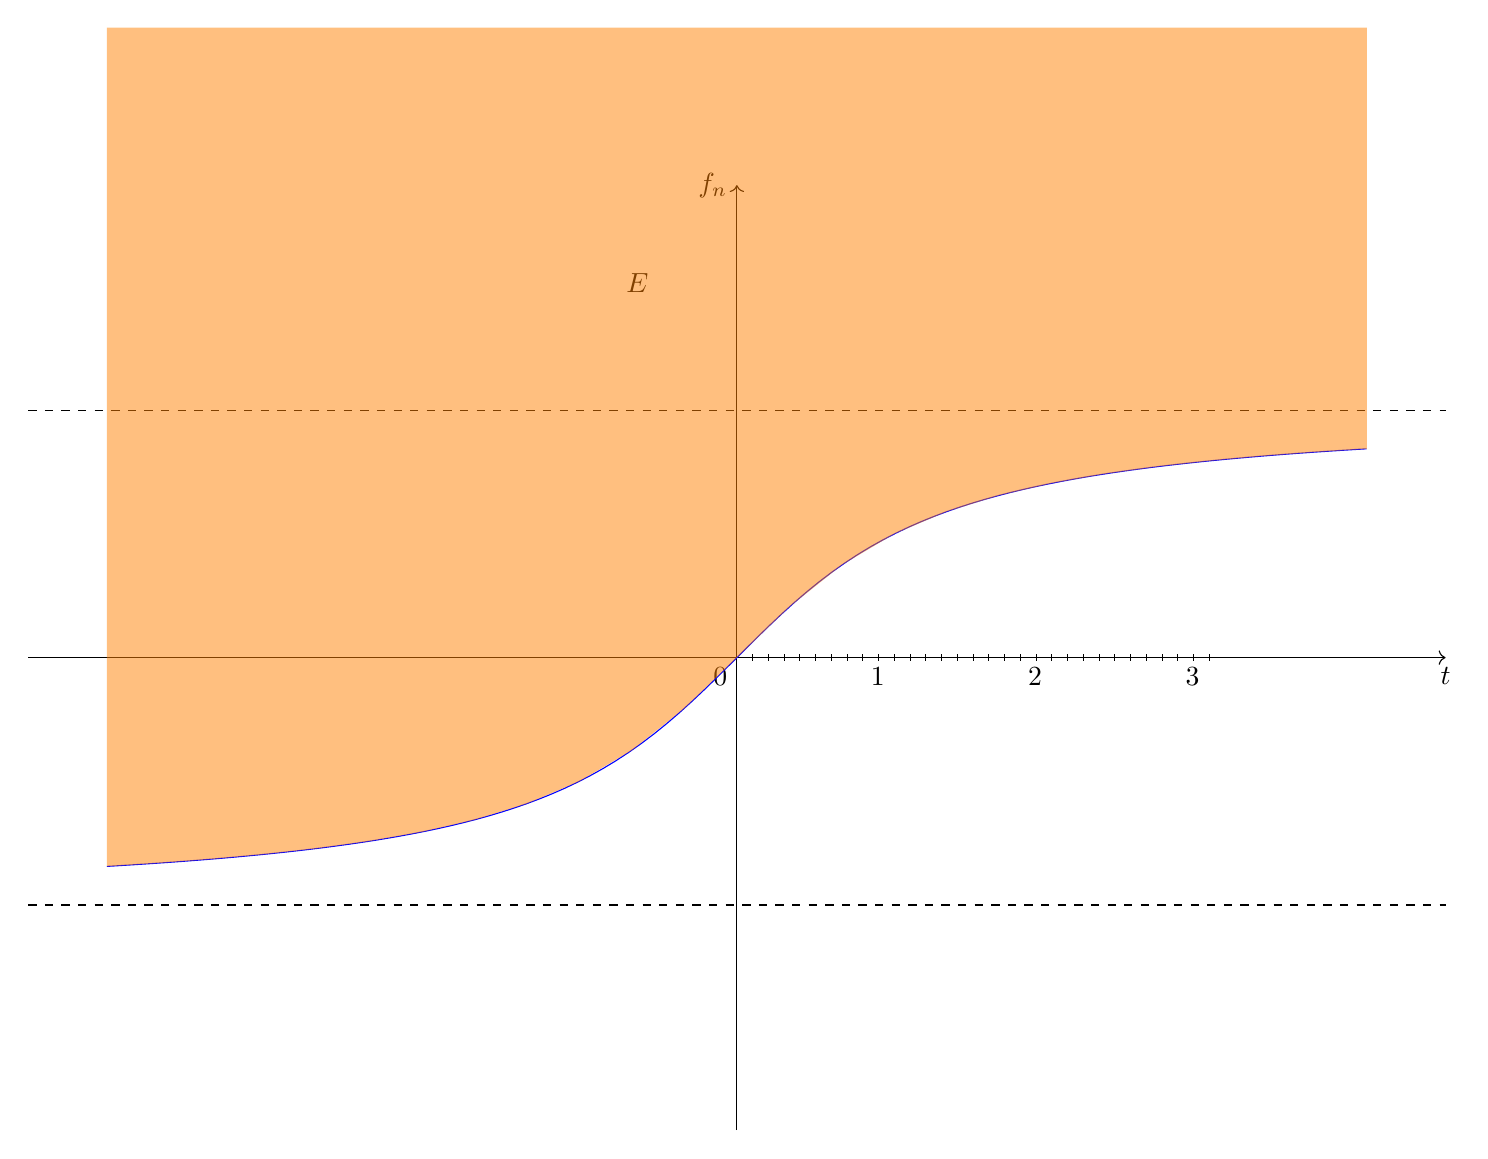
\begin{tikzpicture}[scale=2.]
\draw[->] (-4.5,0)--(4.5,0) node[below]{$t$};   
\draw[->] (0,-3)--(0,3)  node[left]{$f_n$};
\draw[dashed] (-4.5,pi/2)--(4.5,pi/2);
\draw[dashed] (-4.5,-pi/2)--(4.5,-pi/2);
\path
(0,0) node[below left]{$0$};
\path
(1,0) node[below left]{$1$};
\path
(2,0) node[below left]{$2$};
\path
(3,0) node[below left]{$3$};
\path
(-0.5,2.5) node[below left]{$E$};
\foreach \i in {0.,0.1, 0.2,...,3.0} \draw (\i,-0.02)--(\i,0.02);
\draw[blue, domain=-4:4., samples=100, variable=\x] plot ({\x}, {rad(atan \x)});
\fill [orange,opacity=0.5, domain=-4:4, variable=\x]
      (-4, 4)
      -- plot ({\x}, {rad(atan \x})
      -- (4, 4)
      -- cycle;
\end{tikzpicture}
\end{center}
\end{figure} \vspace{1 cm}
We can see that $E$ is not bounded so it is not compact. Now we see if it is complete. Consider
$$f(x,y) = y - \arctan(x),$$
we have
$$E = f^{-1}([0, +\infty[).$$
It is a contraimage of a closed set, then $E$ is closed. We know that a closed subset of a complete metric space is complete. Since $\mathbb{R}^2$ is complete, then $E$ is complete.
\clearpage
\section*{Exercise $9$}
Let $X = \mathbb{R}^2$ with the Euclidean distance and let
$$A = [0, 1] \times [0, +\infty[$$
$$B = \{ (x, y) \in \mathbb{R}^2 \qquad \textrm{with} \qquad x^2 + y^2 < 1 \}.$$
Say if $A$ and $B$ with the Euclidean distance are complete.
\section*{Solution}
$A$ is closed and $A \subset \mathbb{R}^2$ that is complete with the Euclidean diastance. Then $A$ is complete.
\begin{figure}[!ht]
\begin{center}
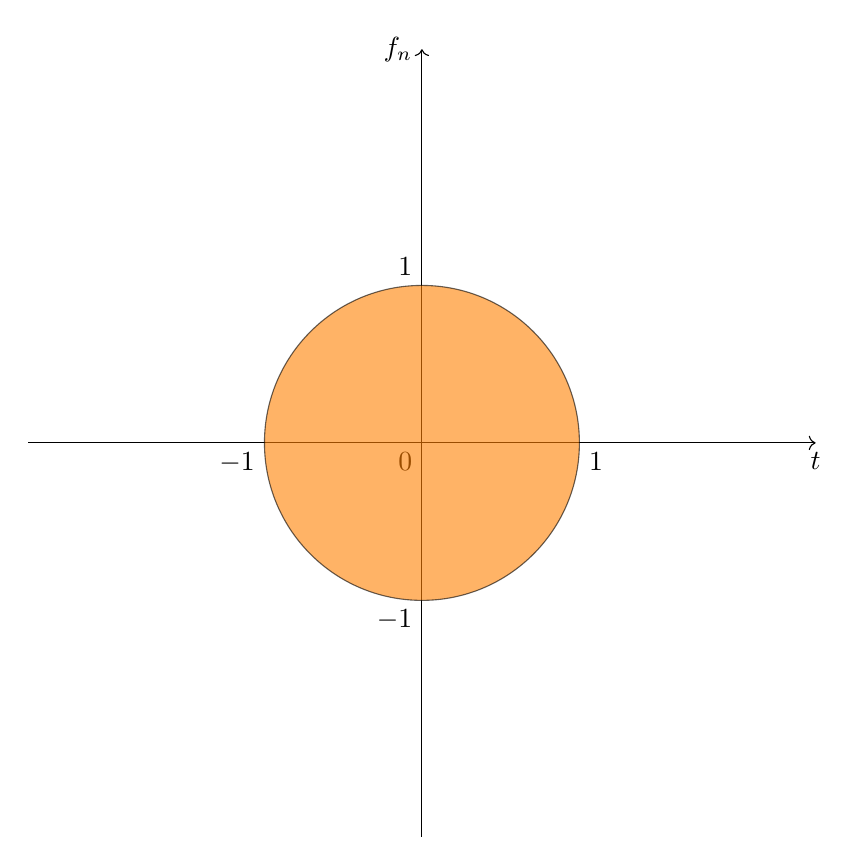
\begin{tikzpicture}[scale=2.]
\draw[->] (-2.5,0)--(2.5,0) node[below]{$t$};   
\draw[->] (0,-2.5)--(0,2.5)  node[left]{$f_n$};
\path
(0,0) node[below left]{$0$};
\path
(1,0) node[below right]{$1$};
\path
(0,1) node[above left]{$1$};
\path
(-1,0) node[below left]{$-1$};
\path
(0,-1) node[below left]{$-1$};
\filldraw[fill=orange, opacity=.6](0,0) circle (1.0);
\end{tikzpicture}
\end{center}
\end{figure} \vspace{1 cm}
$B$ is open, we need to find a Cauchy sequence in $B$ that doesn't converge in $B$. Consider
$$x_n = (1 - \frac{1}{n}, 0) \qquad x_n \in B \qquad \forall n.$$
We have that
$$x_n \rightarrow (1, 0) \qquad \textrm{in} \qquad \mathbb{R}^2,$$
but $(1, 0) \notin B$. We have a sequence that converge in the space, that is a Cauchy sequence, but that doesn't converge in $B$. Then $B$ is not complete.
\clearpage
\section*{Exercise $10$}
Let $(X, d)$ a metric space and $x_n$ a sequence of elements of $X$. Say if the following statements are true or false.
\begin{enumerate}
\item $\lim_{n \rightarrow \infty} d(x_n, x_{n+1}) = 0 \implies x_n \qquad \textrm{bounded}$;
\item $x_n \qquad \textrm{convergent} \implies \lim_{n \rightarrow \infty} d(x_n, x_{n + 1}) = 0$;
\item $x_n \qquad \textrm{Cauchy} \implies \lim_{n \rightarrow \infty} d(x_n, x_{n+1}) = 0$.
\end{enumerate}
\section*{Solution}
\textbf{Point $1$} \par
The fact that $\lim_{n \rightarrow \infty} d(x_n, x_{n+1}) = 0$ doesn't imply that $x_n$ is bounded. Counterexample:
$$x_n = \log{n}$$
$$\lim_{n \rightarrow \infty} d(x_n, x_{n+1}) = \lim_{n \rightarrow \infty} |\log{n+1} - \log{n}| = \lim_{n \rightarrow \infty} |\log{\frac{n + 1}{n}}| = 0.$$
The distances between two consecutive elements become shorter but $x_n$ is not bounded.
$$\sup_{n \in \mathbb{N}} \{ \log{n}, \qquad n \in \mathbb{N} \} = +\infty.$$
Then the first statement is false. \par  
\textbf{Point $2$} \par  
If $x_n$ is convergent then there exists $x_{\infty} \in X$ s.t. :
$$\lim_{n \rightarrow \infty} x_n = x_{\infty}.$$
Then
$$0 \leq d(x_n, x_{n+1}) \leq d(x_n, x_{\infty}) + d(x_{\infty}, x_{n+1}),$$
since $d(x_n, x_{\infty}) \rightarrow 0$, $d(x_{\infty}, x_{n+1}) \rightarrow 0$, then by "the two carabinieri theorem" we have that $d(x_n, x_{n+1}) \rightarrow 0$. \par
\textbf{Point $3$} \par  
$x_n$ is a Cauchy sequence iff
$$\forall \epsilon > 0 \exists \nu \in \mathbb{N} \textrm{s.t.} \forall n, m \geq \nu \in \mathbb{N} \implies d(x_n, x_m) < \epsilon.$$
If we fix $n$, then $m$ can be very far, so is stronger the Cauchy condition with respect to $(x_n, x_{n+1})$, so that:
$$\forall \epsilon > 0 \exists \nu \in \mathbb{N} \textrm{s.t.} \forall n > \nu d(x_n, x_{n+1}) < \epsilon \implies \lim_{n \rightarrow \infty} d(x_n , x_{n+1}) = 0.$$
\clearpage
\section*{Exercise $11$}
Determine as $\alpha$ varies the limit in $(\mathbb{R}^2, d_2)$ of the sequence:
$$x_n = (\frac{1}{n}, (-1)^n \frac{n^{\alpha} - 1}{n^2}.$$
If the limit doesn't exists find eventual convergent subsequences.
\section*{Solution}
A sequence in $\mathbb{R}^2$ is like having two sequences in $\mathbb{R}$:
$$a_n = \frac{1}{n} \rightarrow 0$$
$$b_n = (-1)^n \frac{n^{\alpha} - 1}{n^2} = (-1)^n n^{\alpha - 2} + \frac{(-1)^n}{n^2} \rightarrow 0.$$
\begin{itemize}
\item If $\alpha - 2 < 0$ then $b_n \rightarrow 0$;
\item if $\alpha = 2$ then $b_n \rightarrow \nexists$;
\item if $\alpha - 2 > 0$ then $b_n \rightarrow \nexists$.
\end{itemize}
Then if $\alpha < 2$ then 
$$\lim_{n \rightarrow \infty} x_n = (0, 0)$$
if $\alpha \geq 2$
$$\lim_{n \rightarrow \infty} x_n = \nexists.$$
If we consider $\alpha > 2$ since $|b_n \rightarrow +\infty$ there aren't convergent subsequences.
If $\alpha = 2$ we the subsequence of even indices
$$x_n = (\frac{1}{n}; \frac{n^2 + 1}{n^2}) \rightarrow (0, 1),$$
the subsequence of odd indices:
$$x_n = (\frac{1}{n}; -\frac{n^2 + 1}{n^2}= \rightarrow (0, -1).$$
\clearpage
\section*{Exercise $12$}
Let $(X, d)$ a metric space, $A \subseteq X$, $A \neq \emptyset$, $x_n$ a sequence in $A$ that converges to $x_{\infty} \in X$. Say if the following statements are false or true.
\begin{enumerate}
\item $x_{\infty}$ is an accumulation point for $A$;
\item $x_{\infty} \in \overline{A}$;
\item $x_{\infty} \in \mathring{A}$;
\item $x_{\infty} \in \partial A$. 
\end{enumerate}
\section*{Solution}
\textbf{Point $1$} \par 
The first statement is false. Counterexample:
$$A = [0, 1] \cup \{ 2 \}$$
$$x_n = 2 \qquad \textrm{constant}$$
$$\lim_{n \rightarrow \infty} x_n = x_{\infty} = 2$$
that is not an accumulation point since $2$ is an isolated point for $A$. \par  
\textbf{Point $2$} \par 
If $x_{\infty}$ is an isolated point the statement follows by the point $1$, if $x_{\infty}$ is not an isolated point it will be an accumulation point then the statement trivially follows. So the statement $2$ is true. \par 
\textbf{Point $3$} \par
$x_{\infty} \in \mathring{A}$ is false. Counterexample:
$$A = ]0, 1]$$
$$x_n = \frac{1}{n} \implies x_{\infty} \rightarrow 0 \notin \mathring{A}.$$
\textbf{Point $4$} \par  
$x_{\infty} \in \partial A$ is false. Counterexample:
$$A = ]0, 1[$$
$$x_n = \frac{1}{2} + \frac{1}{n}$$
$$x_n \rightarrow \frac{1}{2}$$
that is not in $\partial A$.
\clearpage
\section*{Exercise $13$}
Show that the metric space $(C^0([0, 1]), d_{\infty})$ is not compact.
\section*{Solution}
Consider
$$f_n(t) = t^n \qquad t \in [0, 1]$$
suppose that there is a subsequence that converges to $f \in C^0([0,1])$:
$$f_{nk} \rightarrow f,$$
that is
$$d_{\infty}(f_{nk}, f) \rightarrow 0, \qquad \forall t \in [0, 1].$$
$$|f_{nk}(t) - f_n(t)| \leq d_{\infty}(f_{nk}, f) \rightarrow 0.$$
If this holds then
$$f_{nk}(t) \rightarrow f_n(t) \qquad \forall t \in [0, 1]$$
$$f_n(t) \rightarrow g(t) = \begin{cases}
								0 \qquad \textrm{if} t \in [0, 1[ \\
								1 \qquad \textrm{if} t = 1
						    \end{cases}$$
If the sequence converge to $g(t)$ then also the subsequences tends to $g(t)$, but $f_n$ can't have convergent subsequences because they must to converge to $g(t) \notin C^0([0, 1])$ because $g(t)$ is not continuous. Then $C^0([0, 1])$ is not compact.
\clearpage
\section*{Exercise $14$}
Consider the sequence
$$f_n(t) = \sqrt{\frac{1 + n^2 t^2}{n}} \qquad \textrm{for} t \in [-1, 1].$$
Show that $f_n \rightarrow f$ with $f(t) = |t|$ with the distance $d_{\infty}$. Furthermore deduce that the space $C^1([-1, 1], d_{\infty})$ is not complete.
\section*{Solution}
$$|f_n(t) - f(t)| = |\frac{\sqrt{1 + n^2 t^2}}{n} - |t| | = | \frac{1}{n \sqrt{1 + n^2 t^2} + n|t|}| \leq \frac{1}{n}$$
Since the denominator is greater or equal to $n$ we have that the fraction is lower or equal to $\frac{1}{n} \qquad \forall t \in [-1, 1]$. Then
$$0 \leq d_{\infty}(f_n, f) \leq \frac{1}{n} \rightarrow 0.$$
Then $f_n \rightarrow f$ is a Cauchy sequence, but $f \notin C^1([-1, 1])$. Then the squence doesn't converge in $(C^1[-1, 1], d_{\infty})$ and so it is not complete.
\clearpage
\section*{Exercise $15$}
Let $X = C^0([0,1])$ with the distance $d_2$. Show that the sequence
$$f_n(t) = \begin{cases}
				0 \qquad \textrm{if} \qquad t \in [0, \frac{1}{2} - \frac{1}{n}[ \\
				\sqrt{2nt +2 - n} \qquad \textrm{if} \qquad t \in [\frac{1}{2} - \frac{1}{n}, \frac{1}{2} \\
				\sqrt{-2n t + 2 + n} \qquad \textrm{if} \qquad t \in [\frac{1}{2}, \frac{1}{2} + \frac{1}{n}[ \\
				0 \qquad \textrm{if} \qquad t \in [\frac{1}{2} + \frac{1}{n}, 1] 
		   \end{cases}$$
\begin{enumerate}
\item converges to the null function in $x=2$:
\item does not converge to the null function in the metric space $(X, d_{\infty})$;
\item admits limit in $(X, d_{\infty})$.
\end{enumerate}
\section*{Solution}
\textbf{Point $1$} \par
We need to verify that $d_2(f_n, 0) \rightarrow 0$ where
$$d_2(f_n, 0) = \sqrt{\int_0^1 |f_n(t)|^2 dt}$$
\begin{figure}[!ht]
\begin{center}
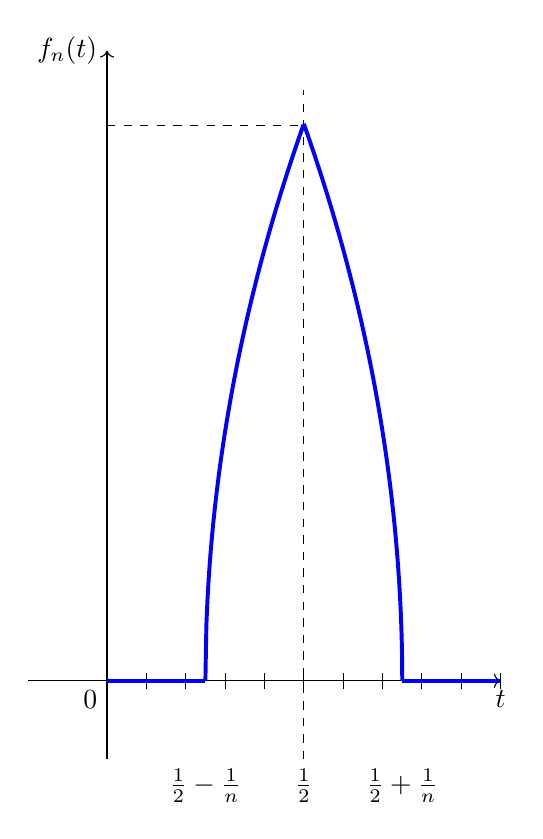
\begin{tikzpicture}[scale=5.]
\draw[->] (-0.2,0)--(1,0) node[below]{$t$};   
\draw[->] (0,-0.2)--(0,1.6)  node[left]{$f_n(t)$};
\draw[dashed] (0,1.41)--(0.5,1.41);
\draw[dashed] (1./2,-0.2)--(0.5,1.5);
\path
(0,0) node[below left]{$0$};
\foreach \i in {0.,0.1, 0.2,...,1.0} \draw (\i,-0.02)--(\i,0.02);
\draw[line width = 0.5 mm,blue, domain=0.:1./4, samples=100, variable=\x] plot ({\x}, {0});
\draw[line width = 0.5 mm,blue, domain=1./4:1./2, samples=100, variable=\x] plot ({\x}, {sqrt(8 * \x - 2)});
\draw[line width = 0.5 mm,blue, domain=1./2:3./4, samples=1000, variable=\x] plot ({\x}, {sqrt(-8 * \x + 6)});
\draw[line width = 0.5 mm,blue, domain=3./4:1., samples=100, variable=\x] plot ({\x}, {0});
\path
(1./4,-0.2) node[below]{$\frac{1}{2} - \frac{1}{n}$};
\path
(0.5,-0.2) node[below]{$\frac{1}{2}$};
\path
(3./4,-0.2) node[below]{$\frac{1}{2} + \frac{1}{n}$};
\end{tikzpicture}
\end{center}
\end{figure}
We have that
$$(d_2(f_n, 0))^2 \leq \frac{2}{n} \rightarrow 0.$$
\textbf{Point $2$} \par  
$$d_{\infty}(f_n, 0) = \sup_{t \in [0,1]} |f_n(t)| = f_n(\frac{1}{2}) = \sqrt{2}.$$
It doesn't tend to zero then it doesn't tend to the null function with the distance $d_{\infty}$.
\textbf{Point $3$} \par 
We suppose that the sequence admits a limit and that
$$\exists g \in X \qquad \textrm{s.t.} \qquad d_{\infty}(f, g) \rightarrow 0.$$
Then
$$\forall t \in [0, 1] \qquad 0 \leq |f_n(t) - g(t)| \leq d_{\infty}(f_n, g)$$
since the "due carabinieri" theorem 
$$\forall t \in [0, 1] \qquad f_n(t) \rightarrow g(t).$$
If $t \neq \frac{1}{2}$ we have that $f_n(t) \rightarrow 0 \implies g(t) = 0$. \par  
If $t = \frac{1}{2} \qquad f_n(t) = \sqrt{2} \implies g(\frac{1}{2}) = \sqrt{2} \implies g \notin X$. Then the limit with $d_{\infty}$ doesn't exist.
\clearpage
\section*{Exercise $16$}
Let $f \in C^1(\mathbb{R}, \mathbb{R})$, $2\pi$-periodic, such that its Fourier series is of the form
$$\sum_{n=3}^{\infty} \alpha_n \sin(n x)$$. Let the Fourier series associated to $f^3$ of the form 
$$\sum_{n=0}^{\infty} a_n \cos(n x) + b_n \sin(n x).$$
Which of the following statements is certainly true?
\begin{enumerate}
\item $b_n = \alpha_n^3 \qquad \forall n$;
\item $a_n = 0 \qquad \forall n$.
\end{enumerate}
\section*{Solution}
Trivially we can see that $f$ is an odd function, then $f^3$ is also an odd function, so that $a_n = 0 \qquad \forall n$ is certainly true. Then
$$\mathcal{F}_{f^3(x)} = \sum_{n = 0}^{+ \infty} b_n \sin(n x).$$
If we consider
$$\alpha_n = \frac{1}{\pi} \int_{-\pi}^{\pi} f(x) \sin(n x) dx$$
$$b_n = \frac{1}{\pi} \int_{-\pi}^{\pi} f^3(x) \sin(n x) dx.$$
Generally is not true that $b_n = \alpha_n^3$. Counterexample:
$$f(x) = \sin(x)$$
$$\alpha_3 = 1 \qquad \textrm{and} \qquad \alpha_n = 0 \qquad \forall n \neq 3.$$
All the terms such as $\sin(4 x), \sin(5 x), \cdots \sin(1000 x)$ have null coefficients.
$$f^3(x) = \sin^3(3 x)$$
$$\alpha_3 = 1$$
$$b_3 = 1^3 ??$$
$$b_3 = \frac{}{} \int_{-\pi}^{\pi} f^3(x) \sin( 3 x) dx = \frac{1}{\pi} \int_{-\pi}^{\pi} \sin^4( 3 x) dx = \frac{1}{\pi} \int_{-\pi}^{\pi} \sin^2(3 x) (1 - \cos^2(3 x) dx $$
$$= \frac{1}{\pi} \sin^2( 3 x) dx - \frac{1}{\pi}\int_{-\pi}^{\pi} \sin^2(3 x) \cos^2(3 x) dx = \star$$
using the duplication and bisection formulas 
$$\sin^2(3 x) = \frac{1 - \cos(6 x)}{2}$$
$$\sin^2(3 x) \cos^2(3 x) = \frac{\sin^2(6 x)}{4} = \frac{1 - \cos(12 x)}{8}$$
$$\star = \frac{1}{\pi}\int_{-\pi}^{\pi} \frac{1 - \cos(6 x)}{2} dx - \frac{1}{\pi}\int_{-\pi}^{\pi} \frac{1 - \cos(12 x)}{8} dx$$
$$= \frac{1}{2 \pi}[x]_{-\pi}^{\pi} - \frac{1}{12 \pi}[\sin(n x)]_{-\pi}^{\pi} - \frac{1}{8 \pi}[x]_{-\pi}^{\pi} + \frac{1}{96 \pi}[\sin(12 x)]_{-\pi}^{\pi} = \frac{3}{4}.$$
Then
$$\alpha_3 = 1 \qquad b_3 = \frac{3}{4} \neq 1^3.$$
\clearpage
\section*{Exercise $17$}
Let $f \in C^1(\mathbb{R}^2, \mathbb{R})^2$ such that $f(3, 6) = (0, 0)$. In a neighborhood of $(3, 1)$, which of the following statements are certainly true?
\begin{enumerate}
\item $\exists \alpha \in \mathbb{R}$ such that $x \mapsto x + \alpha f(x)$ satisfies the hypotheses of the Implicit Function Theorem.
\item $\forall \alpha \in \mathbb{R} \qquad x \mapsto x + \alpha f(x)$ satisfies the hypotheses of the Inverse Function Theorem.
\end{enumerate}
\section*{Solution}
\textbf{Point $1$} \par 
We need to show that the derivative of $f$ in $(3, 1)$ is an invertible matrix. Counterexample: let $\alpha = 0$ and consider a function $g(x) = x \mapsto x$. Let
$$g(x_1, x_2) = (x_1, x_2)$$
$$Dg(x_1, x_2) = \begin{bmatrix}
					1 & 0 \\
					0 & \
				 \end{bmatrix}$$
The determinant $\det Dg = 1 \neq 0$. Then the gradient matrix is invertible
and since it is constant it is also invertible in $(3, 1)$. So the first statement is true. \par  
\textbf{Point $2$} \par   
Counterexample. We need to find a function $f$ with two variables such that $Df = 0$, starting from a function $g$ not invertible. Consider
$$g(x_1, x_2) = \begin{bmatrix}
					3 \\
					1
                \end{bmatrix}$$
with $\alpha = 1$, we have
$$Dg(x_1, x_2) = \begin{bmatrix}
					0 & 0 \\
					0 & 0
				\end{bmatrix}$$
The gradient matrix $Dg$ is not invertible and it doesn't satisfy the Inverse Function Theorem hypotheses.
$$\begin{bmatrix}
	3 \\
	1
\end{bmatrix} = \begin{bmatrix}
					x + f_1(x) \\
					y + f_2(y)
				\end{bmatrix}$$
$$f_1(x, y) = 3 - x$$
$$f_2(x, y) = 1 - y$$
$$f(3, 1) = \begin{bmatrix}
				0 \\
				0
			\end{bmatrix}$$
Then the second statement is false.
\clearpage
\section*{Exercise $18$}
Let $f \in C^2(\mathbb{R}^2, \mathbb{R})$ such that $f(1, 2) = 0$ and consider a neighborhood of $(1, 2)$. Which of the following statements are certainly true?
\begin{enumerate}
\item $\forall \alpha \in \mathbb{R} \qquad x + \alpha f(x, y) + y - 3 = 0$ satisfies the Implicit Function Theorem hypotheses;
\item $\exists \alpha \in \mathbb{R}$ such that $x + \alpha f(x, y) + y - 3 = 0$ satisfies the Implicit Function Theorem hypotheses.
\end{enumerate}
\section*{Solution}
$$g(x, y) = x + \alpha f(x, y) + y - 3$$
$$g(1, 2) = 0$$
$$f \in C^2 \implies g \in C^2$$
We need to verify if
$$\frac{g}{y} (1, 2) \neq 0 ?$$
$$\frac{g}{x} (1, 2) \neq 0 ?$$
\textbf{Point $2$} \par 
We take $\alpha = 0$ so that $g(x, y) = x + y - 3$. Then
$$\frac{\partial g}{\partial y}(1, 2) = 1 \neq 0.$$
Then the first statement is true. \par
\textbf{Point $1$} \par  
We need a counterexample, starting from a function $g(x, y) = x^2 + y^2$ we can consider:
$$g(x, y) = (x - 1)^2 + (y - 2)^2$$
so that
$$\nabla g(1, 2) = [0, 0].$$
We have
$$x + \alpha f(x, y) + y - 3 = (x - 1)^2 + (y - 2)^2.$$
We take $\alpha = 1$.
$$x + f(x, y) + y - 3 = (x - 1)^2 + (y - 2)^2$$
$$f(x, y) = (x - 1)^2 + (y - 2)^2 - x - y + 3$$
$$f(1, 2) = (0, 0)$$
and $f \in C^2$, but
$$\nabla f(1, 2) = [0, 0]$$
so that $f$ is not invertible. Then the second statement is not true.
\clearpage
\section*{Exercise $19$}
Let $f_{\alpha} : \mathbb{R}^2 \rightarrow \mathbb{R}$ given by:
$$f_{\alpha}(x, y) = \begin{cases}
						\frac{|x|^{\alpha} y^2}{\sqrt{4 x^2 + 3 y^2}} \qquad \textrm{if} \qquad x \neq 0 \\
						0 \qquad \textrm{if} \qquad x = 0
					 \end{cases}$$
Studying with respect to $\alpha \in \mathbb{R}$ the differentiability and continuity of $f_{\alpha}$.
\section*{Solution}
\textbf{First: continuity} \par 
We have problems in all the points of the $y$-axis. First we consider the points $(0, b)$ with $b \neq 0$ that is a generic point of the $y$ axis.
$$\lim_{(x, y) \rightarrow (0, b)} \frac{|x|^{\alpha} y^2}{\sqrt{4 x^2 + 3 y^2}} = \frac{b^2}{\sqrt{3 b^2}} \lim_{(x,y) \rightarrow (0,b)} |x|^{\alpha} = \begin{cases}
+\infty \qquad \textrm{if} \qquad \alpha < 0 \\
\frac{b^2}{\sqrt{3 b^2}} \qquad \textrm{if} \qquad \alpha = 0\\
0 \qquad \textrm{if} \qquad \alpha > 0.
\end{cases}$$
Then $f$ is continous in $(0, b)$ with $b \neq 0 \qquad \forall \alpha > 0$.
Now we consider the point $(0, 0)$.
$$\lim_{(x, y) \rightarrow (0, 0)} \frac{|x|^{\alpha} y^2}{\sqrt{4 x^2 + 3 y^2}}$$
in polar coordinates
$$\lim_{\rho \rightarrow 0} \frac{\rho^{\alpha} |\cos \theta|^{\alpha} \rho^2 (\sin^2 \theta)}{\rho \sqrt{4 \cos^2 \theta + 3 \sin^2 \theta}}$$ 
making some additions
$$|\rho^{\alpha + 1} \frac{|\cos \theta|^{\alpha} (\sin^2 \theta)}{\sqrt{4 \cos^2 \theta + 3 \sin^2 \theta}}| \leq \rho^{\alpha + 1} \frac{|\cos \theta|^{\alpha} |\sin^2 \theta|}{\sqrt{3}|\sin \theta|} = \frac{\rho^{\alpha + 1}}{\sqrt{3}} |\cos \theta|^{\alpha} |\sin \theta| \leq \frac{\rho^{\alpha + 1}}{\sqrt{3}}$$
uniformly in $\theta$. \par  
If $\alpha > 0$ then $L = 0$ uniformly in $\theta$. \par 
If $\alpha \leq -1$ then $L = \nexists$. \par   
Remains the case $-1 < \alpha < 0$.
$$\lim_{\rho \rightarrow 0} \frac{\rho^{\alpha + 1} |\cos \theta|^{\alpha} \sin^2 \theta}{\sqrt{4 \cos^2 \theta + 3 \sin^2 \theta}} = 0$$
this limit is equivalent to
$$\lim_{\rho \rightarrow 0} \rho^{\alpha + 1} h(z) = 0 \qquad \forall \theta \neq \frac{\pi}{2} \quad \frac{3\pi}{2}$$
but the limit is not uniform since it is not possible to increase the function. Then for $-1 < \alpha < 0$ the limit goes to $+\infty$. The local boundedness theorem is violated. \par 
Then $f$ is continuous for $\alpha \geq 0$, $f$ is continuous in $(0, b)$ for $\alpha \geq 0$. \par 
\textbf{Second: differentiability} \par 
We consider the points $(0, b)$ with $b \neq 0$ and with $\alpha > 0$.
$$\frac{\partial f}{\partial x} (0, b) = \lim_{t \rightarrow 0} \frac{f(t, b) + f(0, b)}{t} = \lim_{t \rightarrow 0} \frac{|t|^{\alpha} b^2}{\sqrt{4 t^2 + 3 b^2}} \frac{1}{t} = \begin{cases}
						\nexists \qquad \textrm{if} \qquad \alpha < 1 \\
						\nexists \qquad \textrm{if} \qquad \alpha = 1 \\
						0 \qquad \textrm{if} \qquad \alpha > 1
					\end{cases}$$
$$\frac{\partial f}{\partial y}(0, b) = \lim_{t \rightarrow 0} \frac{f(0, b + t) - f(0, b)}{t} = \lim_{t \rightarrow 0} \frac{0}{t} = 0.$$
Now we consider the case $\alpha > 1$ and show if $f$ is differentiable. For $\alpha > 1$, $\nabla f(0, 0) = [0, 0]$. 
$$\lim_{(h, k) \rightarrow (0, 0)} \frac{f(h, b + k) - f(0, b) - \nabla f(0, b) \begin{bmatrix} h\\ k \end{bmatrix}}{\sqrt{h^2 + k^2}} = \lim_{(h, k) \rightarrow (0, 0)} \frac{|h|^{\alpha}(b + k)^2}{\sqrt{4 h^2 + 3(b + k)^2} \sqrt{h^2 + k^2}}$$
$$=\lim_{\rho \rightarrow 0} \frac{\rho^{\alpha -1} |\cos \theta|^{\alpha} (b + \rho \sin \theta)^2}{\sqrt{4 \rho^2 \cos^2 \theta + 3 (b + \rho \sin \theta)^2}}= 0 \qquad \forall \theta.$$
Now we show if it is uniformly.
$$|\frac{\rho^{\alpha - 1} |\cos \theta|^{\alpha} (b + \rho \sin \theta)^2}{\sqrt{4 \rho^2 \cos^2 \theta + 3(b + \rho \sin \theta)^2}}| \leq \rho^{\alpha -1} \frac{|b + \rho \sin \theta|}{\sqrt{3}} \leq \rho^{\alpha - 1} \frac{|b| + \rho}{\sqrt{3}}.$$
The right term doesn't depend on $theta$ so the limit is uniform in $\theta$. If $\alpha > 1$ $f$ is differentiable in $(0, b)$ with $b \neq 0$. Now we consider the case $\alpha \geq 0$ in $(0,0)$.
$$\frac{\partial f}{\partial x}(0, 0) = \lim_{t \rightarrow 0} \frac{f(t, 0) - f(0,0)}{t} = \lim_{t \rightarrow 0}\frac{0}{t} = 0$$
$$\frac{\partial f}{\partial y}(0, 0) = \lim_{t \rightarrow 0} \frac{f(0, t) - f(0,0)}{t} = \lim_{t \rightarrow 0}\frac{0}{t} = 0$$
$$\lim_{(h, k) \rightarrow (0,0)} \frac{f(h, k) - f(0, 0) - \nabla f(0, 0) \begin{bmatrix} h\\ k \end{bmatrix}}{\sqrt{h^2 + k^2}} = \lim_{(h, k) \rightarrow (0,0)} \frac{f(h, k)}{\sqrt{h^2 + k^2}} = \lim_{(h, k) \rightarrow (0,0)} \frac{|h|^{\alpha} k^2}{\sqrt{4 h^2 + 3 k^2} \sqrt{h^2 + k^2}}$$
if $\alpha = 0$ the limit is
$$\lim_{(h, k) \rightarrow (0,0)} \frac{k^2}{\sqrt{4 h^2 + 3 k^2} \sqrt{h^2 + k^2}} = \nexists.$$
If $\alpha > 0$ in polar coordinates:
$$\lim_{\rho \rightarrow 0} \frac{\rho^{\alpha} |\cos \theta|^{\alpha} \rho^2 (\sin^2 \theta)}{\rho \rho \sqrt{4 \cos^2 \theta + 3 \sin^2 \theta}} = 0 \qquad \forall \theta.$$
Now we show if it is uniform in $\theta$.
$$|\frac{\rho^{\alpha} |\cos \theta|^{\alpha} \sin^2 \theta}{\sqrt{4 \cos^2 \theta + 3 \sin^2 \theta}}| \leq \rho^{\alpha} \frac{|\cos \theta|^{\alpha} \sin^2 \theta}{\sqrt{3 \sin^2 \theta}} = \frac{\rho^{\alpha} |\cos \theta|^{\alpha} |\sin^2 \theta|}{\sqrt{3} \sin \theta} = \rho^2 \frac{|\cos \theta|^{\alpha} |\sin \theta|}{\sqrt{3}} \leq \frac{\rho^2}{\sqrt{3}}.$$
It is uniform in $\theta$. Then $L = 0$ uniformly in $\theta$. \par  
Then $f$ is differentiable in the origin for $\alpha > 0$.
\clearpage
\section*{Exercise $20$}
Let $A \subseteq \mathbb{R}^n$ open and $f: A \rightarrow \mathbb{R}^m$ differentiable on $A$. Show that:
\begin{enumerate}
\item if $A$ is convex and $\norm{Df(x)} \leq L \qquad \forall x 	in A$ then $f$ is Lip;
\item if $f$ is Lip with constant $L$ then $\norm{Df(x)} \leq L \qquad \forall x \in A$.
\end{enumerate}
\section*{Solution}
\textbf{Point $1$} \par 
We apply the Finite Accretion Theorem. If $A$ is convex, then
$$\forall x'', x' \in A \qquad \norm{f(x'') - f(x')} \leq \sup_{\xi \in A} \norm{Df(\xi)} \norm{x'' - x'} \leq \star$$
since $\norm{Df(x)} \leq L$ then also the $\sup \leq L$, then
$$\star \leq L \norm{x'' - x'}$$
then $f$ is Lip. \par   
\textbf{Point $2$} \par   
Let $x \in A$ , $v \in \mathbb{R}^m$, $t \in \mathbb{R}$.
$$\norm{f(x + tv) - f(x)} \leq L \norm{t v} = L |t| \norm{v}$$
$$\frac{\norm{f(x + tv) - f(x)}}{t} \leq L \norm{v}.$$
Since $f$ is differentiable and derivable, the limit exists, so passing to the limit for $t \rightarrow 0$ we obtain:
$$\norm{Df(x) \cdot v} \leq L \norm{v}.$$
Now we take all the vectors for norm equal to $1$:
$$w \in \mathbb{R}^n \qquad \norm{w} = 1$$
then
$$\norm{Df(x) \cdot w } \leq L,$$
if it is valid for all the previous vectors we obtain
$$\sup_{w \in \mathbb{R}^n, \qquad \norm{w} = 1} \norm{Df(x) w} \leq L$$
then
$$\norm{Df(x)} \leq L.$$
\clearpage





\end{document}